\documentclass{article}
\usepackage{amsmath,amsthm,amssymb,tikz,txfonts,showlabels,hyperref,mathrsfs, float}
\usepackage[linesnumbered,ruled,vlined]{algorithm2e}
\usepackage[utf8]{inputenc}
\usepackage{xcolor}
\newcommand{\red}[1]{\textcolor{red}{#1}} % defines \red{}

\newtheorem{thm}{Theorem}
\newtheorem*{thm*}{Theorem}
\newtheorem{cor}{Corollary}
\newtheorem*{cor*}{Corollary}
\newtheorem{defn}{Definition}
\newtheorem*{defn*}{Definition}
\newtheorem{lem}{Lemma}
\newtheorem*{lem*}{Lemma}
\newtheorem{rem}{Remark}
\newtheorem*{rem*}{Remark}
\newtheorem*{prop*}{Proposition}
\newtheorem{prop}{Proposition}

\SetKwInput{KwInput}{Input}                % Set the Input
\SetKwInput{KwOutput}{Output}     
\SetKwComment{Comment}{/* }{ */}

\newcommand{\set}[1]{\{#1\}}
\newcommand{\R}{\mathbb{R}}
\newcommand{\C}{\mathbb{C}}
\newcommand{\Z}{\mathbb{Z}}
\newcommand{\N}{\mathbb{N}}
\newcommand{\Q}{\mathbb{Q}}
\newcommand{\F}{\mathbb{F}}
\newcommand{\slim}{\lim_{n\rightarrow\infty}}
\newcommand{\spn}[1]{\text{span}({#1})}
\newcommand{\tr}{\text{tr}}
\newcommand{\mc}[1]{\mathcal{#1}}
\newcommand{\brac}[1]{\left({#1}\right)}
\newcommand{\sbrac}[1]{\left[{#1}\right]}
\newcommand{\mat}[1]{\begin{pmatrix}#1\end{pmatrix}}
\newcommand{\dmat}[1]{\begin{vmatrix}#1\end{vmatrix}}
\newcommand{\cis}[1]{\cos(#1)+i\sin(#1)}
\newcommand{\ff}[1]{\mathbf{#1}}
\renewcommand{\vec}[1]{\ff{#1}}
\newcommand{\diagram}[1]{\begin{center}\includegraphics*[scale = 0.4]{#1}\end{center}}
\newcommand{\question}[1]{\newpage\textbf{Question #1}~\\}
\newcommand{\vat}[1]{\ff{\hat{#1}}}
\renewcommand{\d}[1]{\:d#1}
\renewcommand{\i}{\vat{i}}
\renewcommand{\j}{\vat{j}}
\renewcommand{\k}{\vat{k}}
\renewcommand{\empty}{\varnothing}
\renewcommand{\epsilon}{\varepsilon}
\newcommand{\reason}[1]{\tag*{(#1)}}
\renewcommand{\|}{\biggr|}
\newcommand{\dx}{\d x}
\newcommand{\dy}{\d y}
\newcommand{\dz}{\d z}
\newcommand{\ds}{\d s}
\newcommand{\dt}{\d t}
\newcommand{\dr}{\d \vec r}
\newcommand{\inner}[1]{\langle #1\rangle}
\newcommand{\norm}[1]{\|\| #1 \|\|}
\newcommand{\jaco}[2]{\frac{\partial (#1)}{\partial {#2}}}

\title{Documentation}

\begin{document}
\maketitle
    \section{Experimental Setup}
    This experiment involves running four non-conflicting aggregators, namely MGDA, DualProj, UPGrad, and Nash-MTL, on synthetic problems VLMOP2, Omnitest, and ZDT3 with initial seeds 24, 42, 48, 100, and 123. The three problems are defined as such\\
    \textbf{VLMOP2.} 
    \begin{align*}
    \text{Minimize} \quad & f_1(\mathbf{x}) = 1 - \exp\left(-\sum_{i=1}^n \left(x_i - \frac{1}{\sqrt{n}}\right)^2\right), \\
    & f_2(\mathbf{x}) = 1 - \exp\left(-\sum_{i=1}^n \left(x_i + \frac{1}{\sqrt{n}}\right)^2\right), \\
    \text{subject to} \quad & -2.0 \leq x_i \leq 2.0, \quad i = 1, \dots, n,
    \end{align*}
    where \(\mathbf{x} = (x_1, \dots, x_n) \in \mathbb{R}^n\).

    \textbf{ZDT3.} 
    \begin{align*}
    \text{Minimize} \quad & f_1(\mathbf{x}) = x_1, \\
    & f_2(\mathbf{x}) = g(\mathbf{x}) \cdot \left(1 - \sqrt{\frac{x_1}{g(\mathbf{x})}} - \frac{x_1}{g(\mathbf{x})} \sin(10\pi x_1)\right), \\
    \text{where} \quad & g(\mathbf{x}) = 1 + 9 \cdot \frac{1}{n-1} \sum_{i=2}^n x_i, \\
    \text{subject to} \quad & 0.0 \leq x_i \leq 1.0, \quad i = 1, \dots, n,
    \end{align*}
    where \(\mathbf{x} = (x_1, \dots, x_n) \in \mathbb{R}^n\).

    \textbf{Omnitest.} 
    \begin{align*}
    \text{Minimize} \quad & f_1(\mathbf{x}) = \sum_{i=1}^n \sin(\pi x_i), \\
    & f_2(\mathbf{x}) = \sum_{i=1}^n \cos(\pi x_i), \\
    \text{subject to} \quad & 0 \leq x_i \leq 6, \quad i = 1, \dots, n,
    \end{align*}
    where \(\mathbf{x} = (x_1, \dots, x_n) \in \mathbb{R}^n\).
    
    For each aggregator, we will first run the each algorithm without any normalisation on the descent direction. Then, the algorithms will be ran again, this time with the normalisation $d' = d / ||\alpha||_1$, where $\alpha$ is the weighting vector computed by the aggregators. The performance of the algorithm with and without the normalisation will be compared.\\
    ~
    The descent algorithm involve three stopping criteria: Either 1.) the number of maximum iteration has been reached (max iter = 10000), 2.) the sequence $x_t$ remains constant, or 3.) the norm of the descent direction provided by MGDA at the current point is smaller than $\epsilon$. The third criteria would need some more elusidation.\\
    As mentioned in, since the descent direction of MGDA is defined as
    \begin{equation*}
        d^t_{MGDA} = J^T \alpha\text{, where }\alpha \in\arg\min_{\lambda\in\Delta}||\lambda^T JJ^T\lambda||
    \end{equation*}
    Simultaneously, Pareto Stationarity is defined as a point $x$ where $J^T\lambda$ for some $\lambda\in \Delta$. This means $||d^t_{MGDA}||$ can be used as a metric to decide whether Pareto Stationarity has been reached at a point $x$. Consequently, we will include $||d^t_{MGDA}|| < \epsilon$ as our stopping criteria for all aggregators. 
    \section{Multiple Gradient Descent Algorithms (MGDA)}
    To prevent the Gramian $G = JJ^T$ not being full rank due to numerical error, we use the Frank-Wolfe algorithm to compute the descent direction instead.\\
    ~
    Since MGDA requires $||\alpha||_1 = 1$ by design, it is expected that the normalised descent direction is completely idendical to the original MGDA descent direction.\\
    In synthetic problem VLMOP2 and Omnitest, MGDA converges rather smoothly to the Pareto front for all seeds. Despite the seqeunce $x_t$ hits the boundary of the feasible region of Omnitest several times (indicated by the red dots in the figure), MGDA is still able to reguide the sequence to the Pareto front, showing the robustness of the algorithm. In contrast, ZDT3 is relatively more difficult for MGDA, the loss curve were more jagged due to the $x_t$ hitting the boundary of the feasible region. However, the algorithm is still able to converge to the Pareto front. Generally speaking, MGDA is the most robust of all tested aggregators.\\
    \section{DualProj and UPGrad}
    Since the behaviour of DualProj and UPGrad are similar, we will group them into the same section.\\
    In general, the two aggregators performed fairly well in VLMOP2, as the descent algorithm managed to converge to Pareto Stationarity under both aggreators for all seeds. Difficulties arises in Omnitest. In cases where the descent algorithm hits the boundary of the feasible region (random seed 24, 48, 100), the algorithm converge to a non-Pareto stationary point at the boundary. Though in cases where the algorithm does not reach the boundary, it always converge to Pareto stationary. However, ZDT3 is extremely difficult for both aggregators. The descent algorithms hit the boundary in all cases and converges to a non-Pareto stationary point at the boundary.\\
    Comparing across different synthetic problems, we observe that with normalisation, the algorithm tend to converge slower than without normalisation, though the normalised and unnormalised version of the descent algorithm always converge to the same point. As a result of slower convergence, sudden jumps in the course of iteration could be smoothed out. For example, when UPGrad is tested on ZDT3 with random seed 123, a sudden jump in the norm of $d$ can be seen if no normalisation is applied. After applying normalisation, the sudden jump became a smooth peak. In general, the two aggregators is less robust than MGDA, but have better performance than Nash-MTL.
    \section{Nash-MTL}
    In , the weighting vector $\alpha$ is obtained by solving 
    \begin{equation*}
        J^TJ\alpha = \frac{1}{\alpha}, \text{ where } 1/\alpha = \mat{1/\alpha_1 & 1/\alpha_2 & \cdots & 1/\alpha_n}^T
    \end{equation*}
    But since there are no direct way to solve the equation numerically, it needs to be translated into the minimization problem 
    \begin{gather*}
        \text{Minimise } \nabla \varphi(\alpha_{t-1})^T (\alpha_t - \alpha_{t-1}) + \sum_i \beta_i(\alpha)\tag{$\star$}\\
        \text{with constraints}
            -\varphi_i(\alpha_t) \leq 0, \quad \alpha_t^i \geq 0,
    \end{gather*}
    To improve accuracy, we will run the quadratic solver several times, each time substituting the $\alpha$ obtained from the last iteration as $\alpha_0$.\\
    However, empirical experiments showed that the $\alpha$ resulting from the minimization problem often mismatch. For example, in figure \ref{nash_mtl_exp_1}, Nash-MTL was tested on the VLMOP2 and Omnitest. From the figures, one can see that some loss functions increased abruptly in the course of minimising----which should not happen as Nash-MTL is designed to be non-conflicting. To explain such strange behaviour, we used the metric $||G^TG \alpha - 1/\alpha||_\infty$ to measure the deviation of the computed value of $\alpha$ from the theoretical value.\\

    In theory, $\alpha$ is the solution to the equation $G^T G \alpha = 1/\alpha$. Then ideally, $||G^TG \alpha - 1/\alpha||_\infty$ should remain a constant zero. However, it is clear from the figures this is not the case. Two trends can be observed from the measure $||G^T G \alpha - 1/\alpha||_\infty$. First, generally speaking, measure starts from a non-zero value, then gradually drops to zero in the course of minimization. Second, in places where one of the loss functions meets an abrupt increase, the measure also increases abruptly.\\

    The first trend is expected since the minimization problem apporoximates $\varphi$ with a first order Taylor polynomial, its value deviated from the actual objective function $\varphi$. In carrying out the experiment, the quadratic solver was often unable to solve (*) as the problem occasionally becomes unbounded. The red sections of the curves in figure \ref{nash_mtl_exp_1} are exactly those epochs where (*) is unbounded. 
    \begin{figure}
        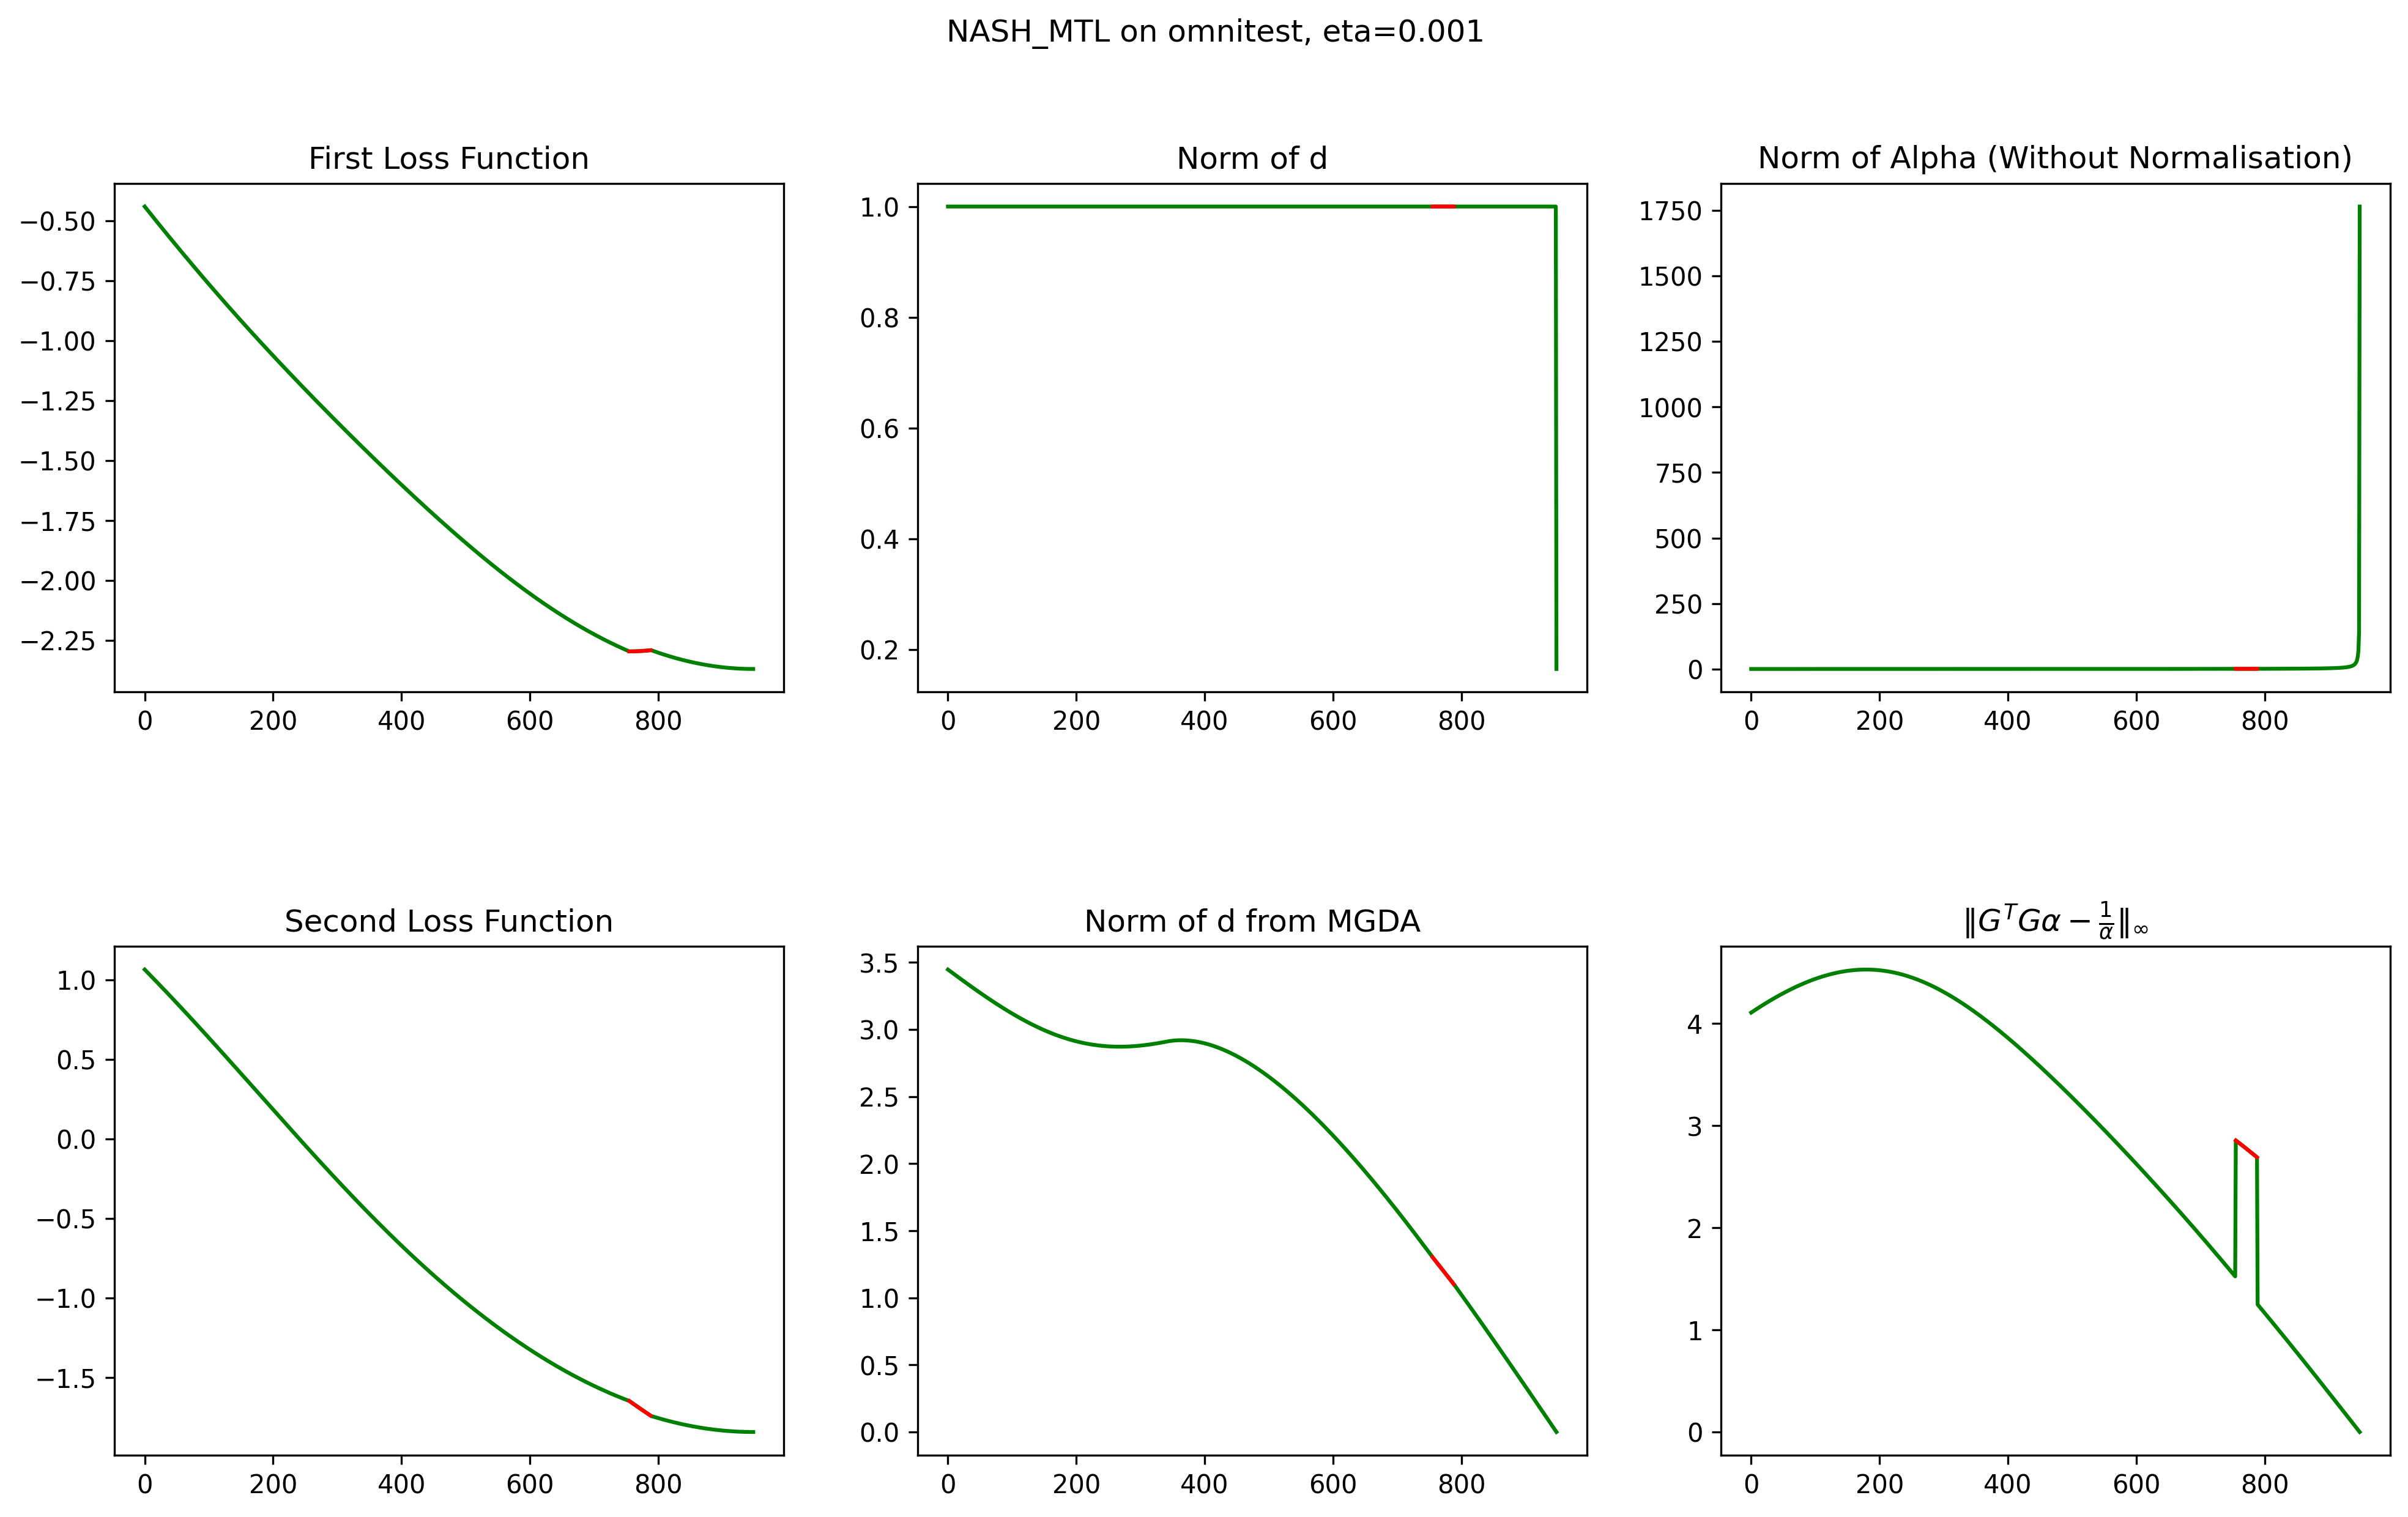
\includegraphics[scale = 0.4]{src/example1.png}
        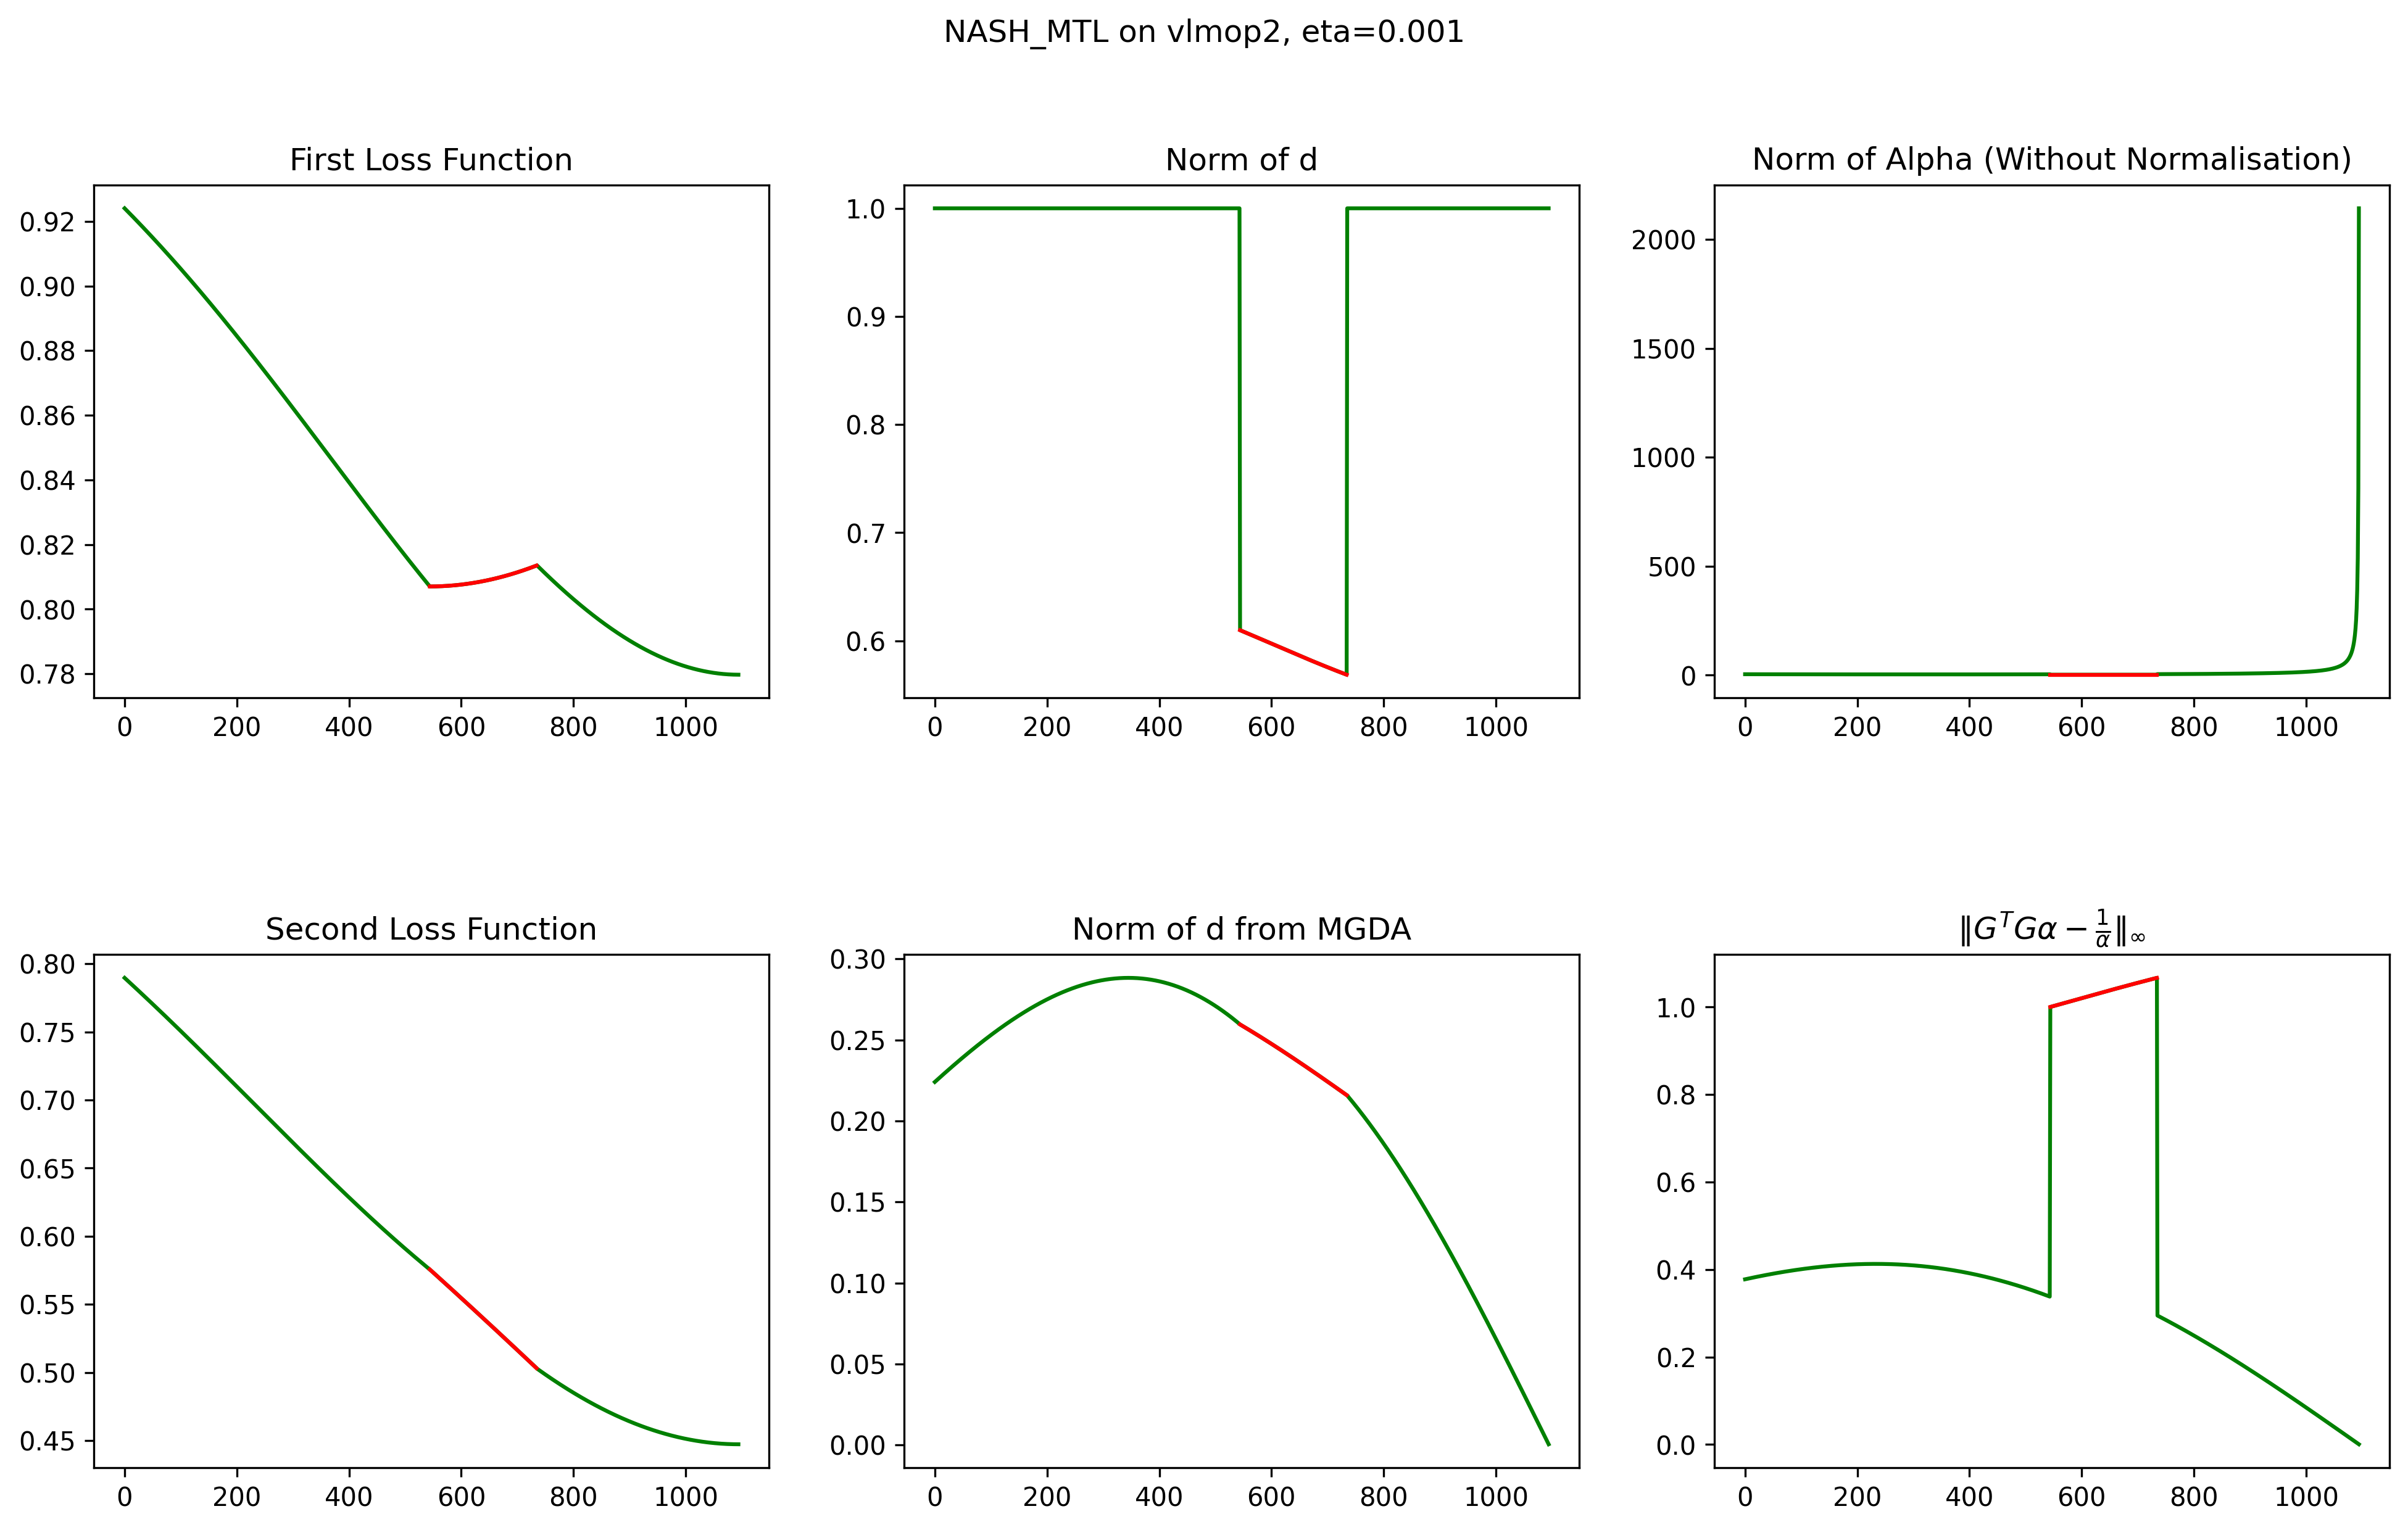
\includegraphics[scale = 0.4]{src/example2.png}
        \caption{Testing Nash-MTL on Omnitest (bottom) and VLMOP2 (top), learning rate = 0.001, max iteration = 15000, seeds = 24. Red section indicates where the minimization problem is unbounded.}\label{nash_mtl_exp_1}
    \end{figure}

    
    Quinton and Rey expressed their doubts with the official implementation both in their paper in their Github repository\footnote{\url{https://github.com/TorchJD/torchjd/blob/main/src/torchjd/aggregation/_nash_mtl.py}}, believing that it may mismatch the desired objective.
    %In the official implementation of Nash-MTL, $\alpha$ is normalised with the following algorithm.
    %\begin{algorithm}[!ht]
    %    \caption{Nash-MTL $\alpha$ normalisation}
    %    \KwInput{$\alpha\in R^n, J\in R^{d\times n}, M\in \R_{>0}$}
    %    \Comment{$M$ is the maximum norm. It is set to $1$ by default.}
    %    \If{$||J^T\alpha||_2 > M$}{
    %        $\alpha\gets \alpha * \frac{M}{||J^T\alpha||_2}$\;
    %    }
    %    \KwOutput{$\alpha$}
    %\end{algorithm}
    %The normalization is not being mentioned in Navon, so it is not being included in our implementation.\\
    %Nevertheless, the motivation for including the normalization can be seen from our experiment. In running Nash-MTL on all three synthetic problems, the norm of $\alpha$ can reach as high as $6000$ which in undesirable. By clipping the magnitude of $\alpha$ to the maximum norm in case $\alpha$ becomes to large, it prevents a $d$ with too large a magnitude. While the normalization method of Nash-MTL's official implementation requires manual determination of the maxmimum norm, our normalsation is more principled and without any need for manually determining a maximum norm.\\
    %In agreement to previous experiments on other aggregators, employing our normalisation results in slower convergence, but also smoother curves. In solving VLMOP2, the quadratic problem is occasionally unsolvable as the minimization is unbounded. This is indicated when sharp turns occurs on the graphs. Although our normalisation cannot prevent this issue, it managed to smooth out all curve present in our plot.\\
    \\
    To improve the performance of Nash-MTL, we try to include more constraints to problem (*) to further restrict the optimization region. It was discovered that including the constraint $||G\alpha||_2^2 \leq n$, where $n$ is the number of tasks, improved the performance of Nash-MTL. The motivation for inclluding this constraint stems from the consideration that $G^TG\alpha = 1/\alpha$ implies the equation that
    \begin{gather*}
        ||d||_2^2 = ||G\alpha||^2_2 = \alpha G^T G \alpha = \alpha^T \frac{1}{\alpha} = n
    \end{gather*}
    After including this constraint, we can see obvious improvement on the performance of Nash-MTL (figure \ref{nash_mtl_exp_2}). 
        \begin{figure}
        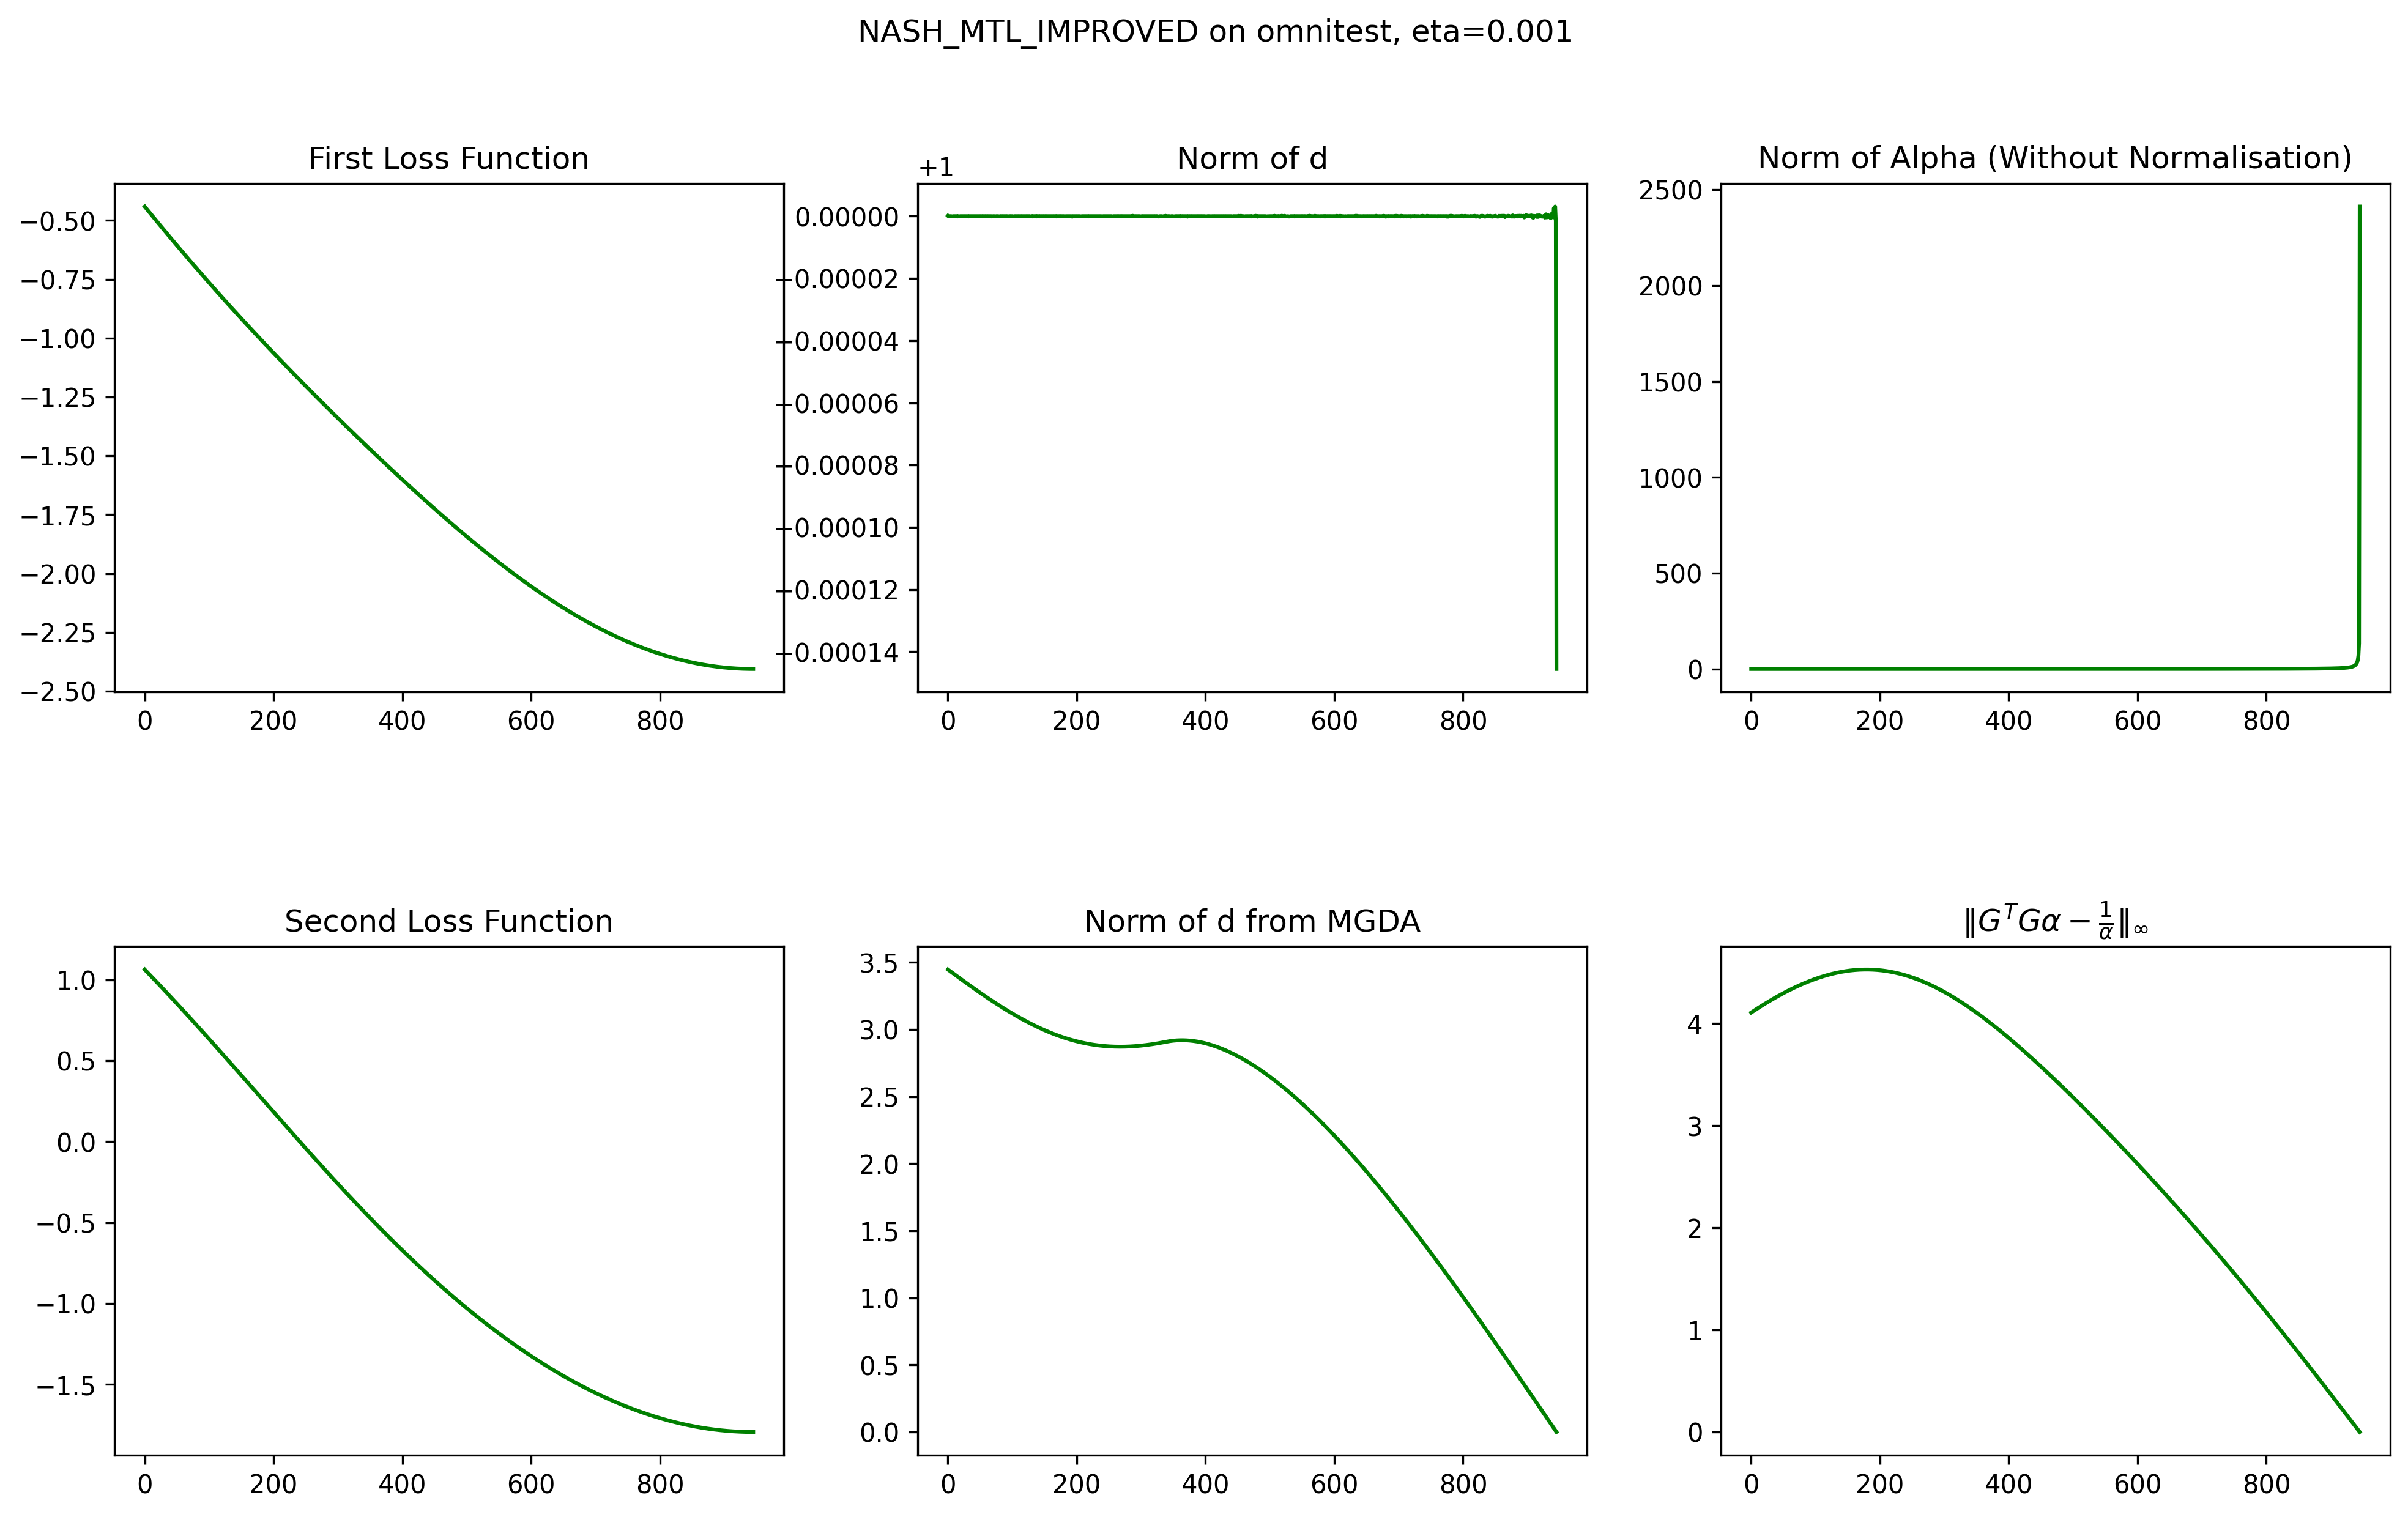
\includegraphics[scale = 0.4]{src/example3.png}
        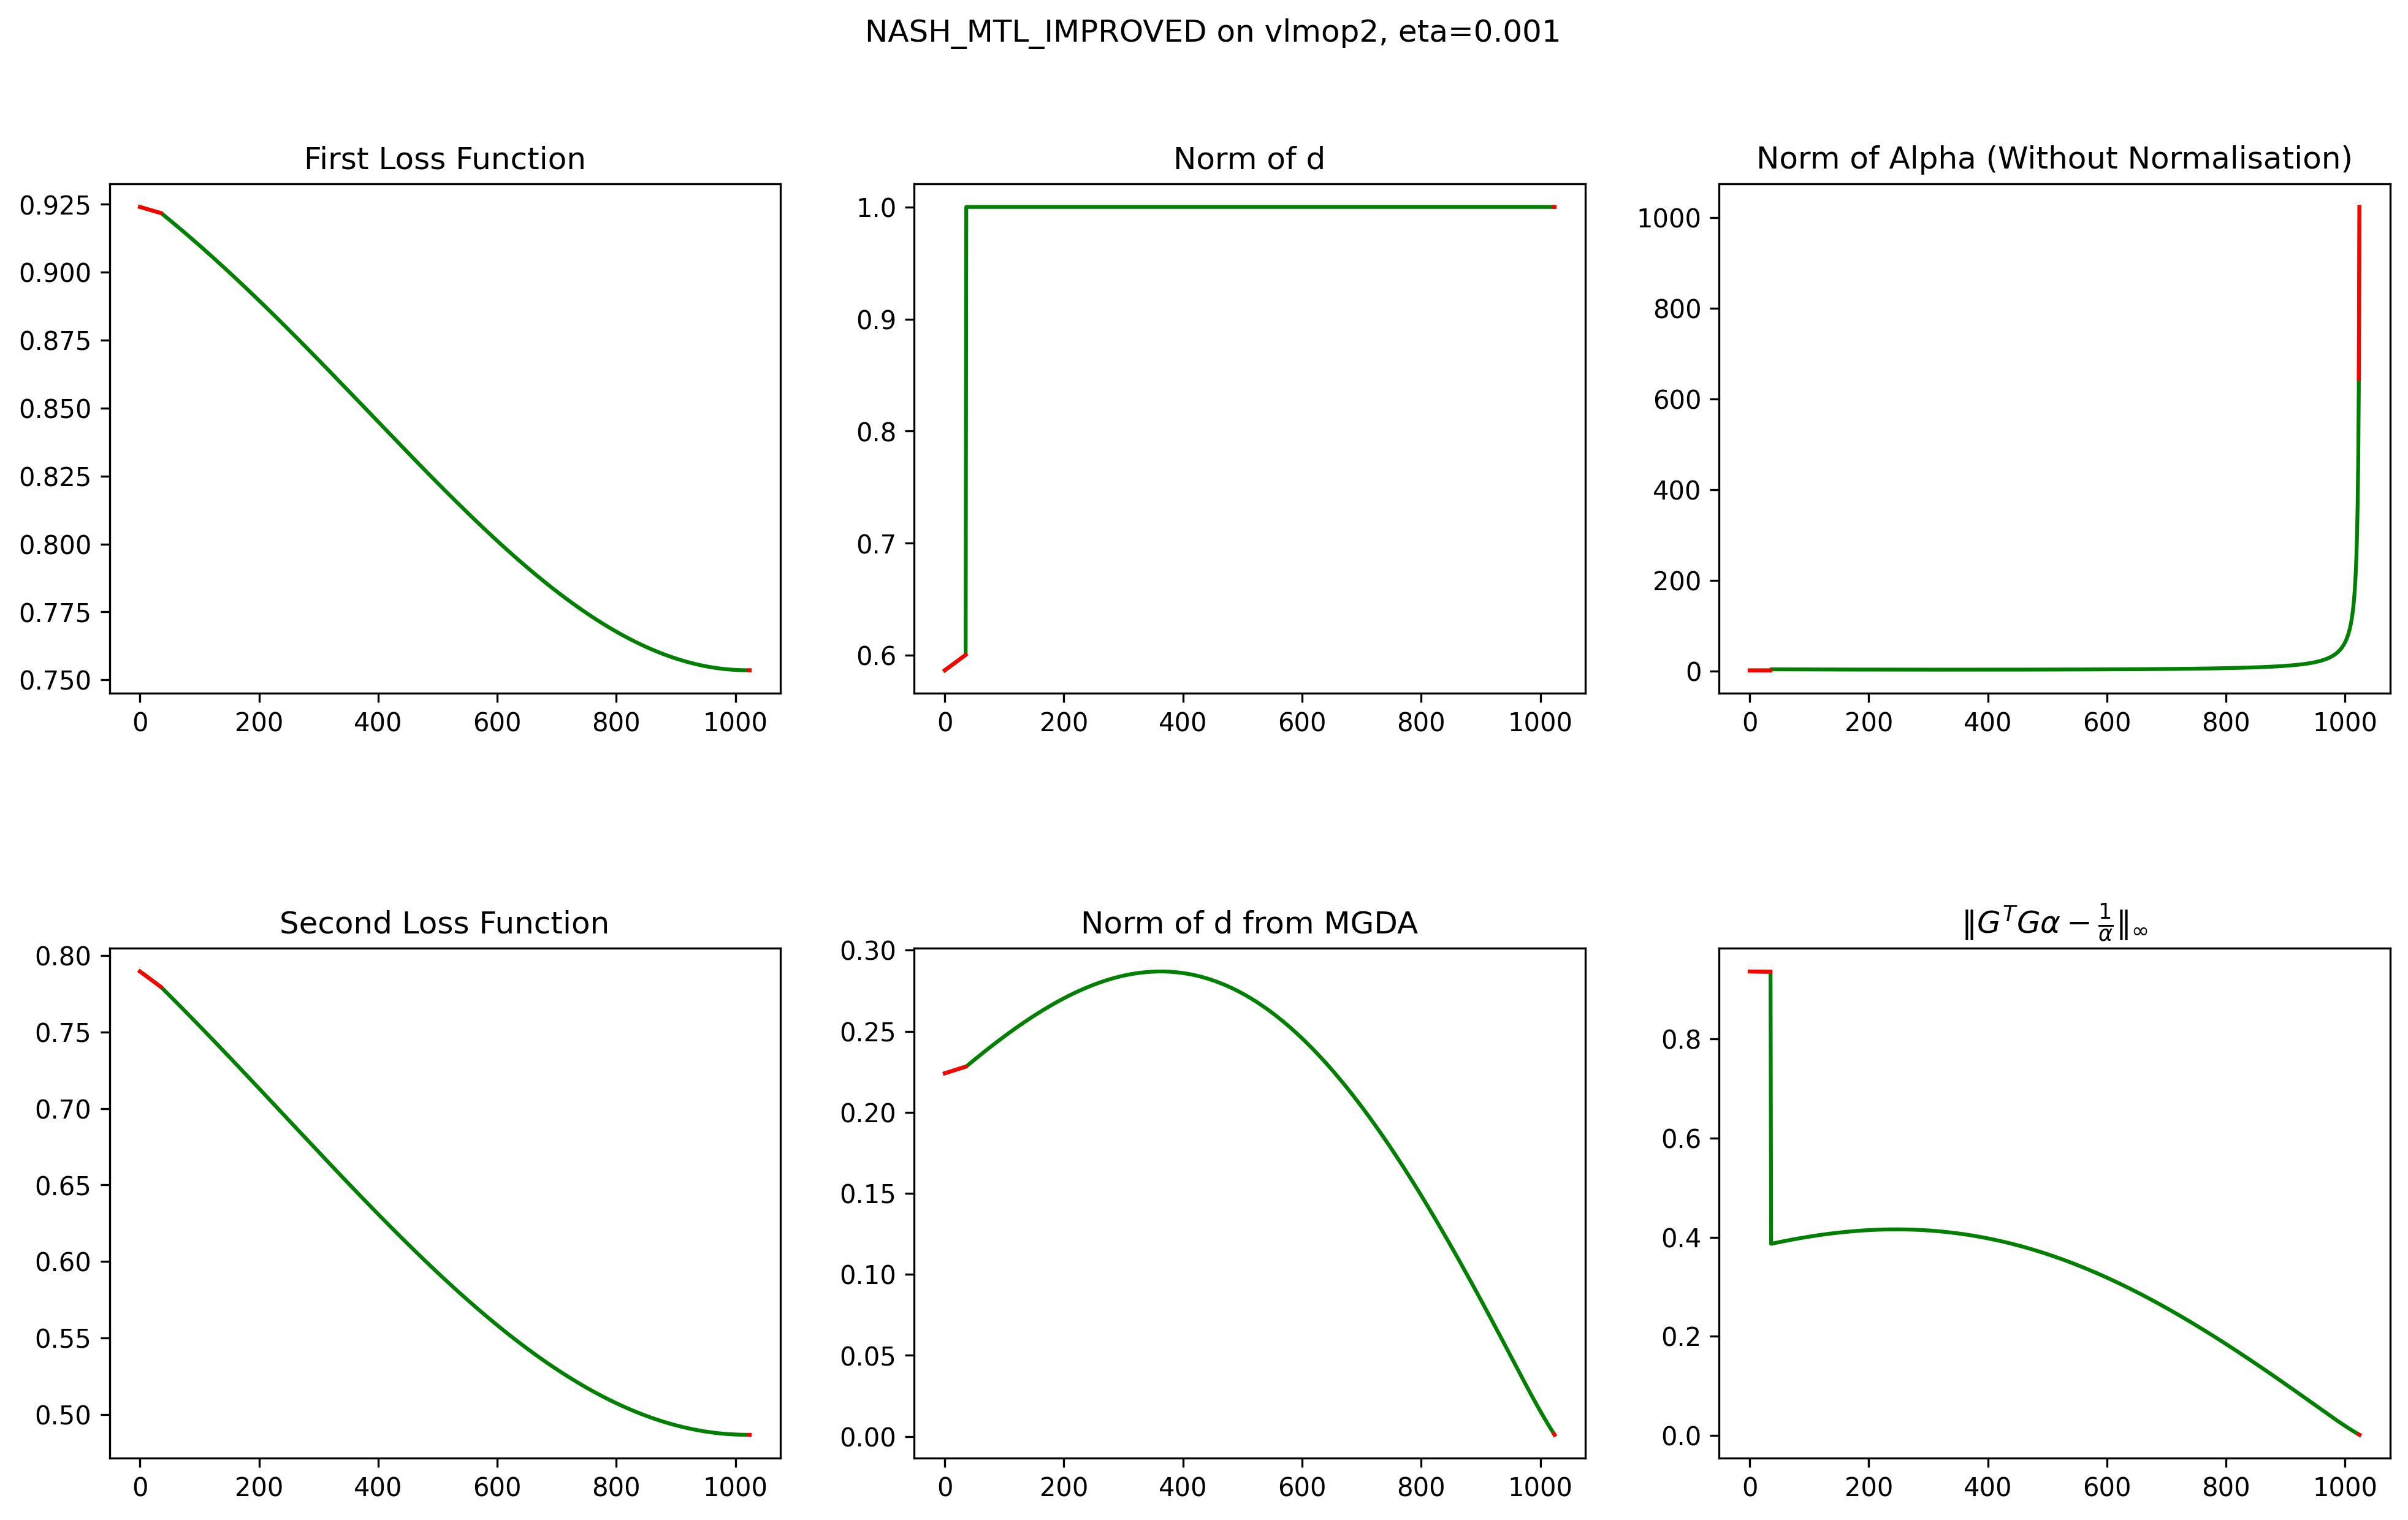
\includegraphics[scale = 0.4]{src/example4.png}
        \caption{Improved Nash-MTL on Omnitest (bottom) and VLMOP2 (top), learning rate = 0.001, max iteration = 15000, seeds = 24. Red section indicates where the minimization problem is unbounded.}\label{nash_mtl_exp_2}
    \end{figure}   
    However, the improved Nash-MTL is not perfect. Figure \ref{nash_mtl_exp_2} shows unboundedness is still possible, though they occur significantly less frequently.\\
    ~\\
    In addition to the additional constraint mentioned above, we introduce one more improvement to Nash-MTL. From figure \ref{nash_mtl_exp_3}, one can see the measure to Pareto Stationarity remains flat from around the 1400th iteration and onwards. However, the measure has not dropped below to pre-determined tolorance ($10^{-2}$), causing the algoirhtm to continue running until the maximum number of iteration has been reached (set to 2000 specifically for this test). Unlike other aggregators such as MGDA, DualProj, and UPGrad, where the norm of $d$ decreases as $x_t$ gets closer to Pareto stationarity, $|d||_2$ remains mostly constant. Thus when $x_t$ get close to Pareto stationarity, $x_t$ tend to oscillate rather than converging to a particular point. We will include learning rate scheduling as a remedy: When the measure from Pareto Stationarity drops below a threshold (set to 0.05 by default), a cyclical learning rate will be adopted. 
    \begin{algorithm}[!ht]
        \caption{Learning rate scheduling for Nash-MTL}
        \KwInput{$d_{Nash-MTL},d_{MGDA}\in \R^{n}, \eta_0,\eta_1,\theta\in \R_{>0}$, $n,T\in \N$}
        \Comment{$d_{Nash-MTL},d_{MGDA}$ are the descent direction provided by Nash-MTL and MGDA respectively. $\theta$ is the threshold value. It is set to $0.05$ by default. $\eta_0, \eta_1$ are the lower bound and upper bound of the cyclical learning rate respectively. When $||d_{MGDA}|\geq\theta$, we set the learning rate to $\eta_1$. Finally, $n$ is the number of epoch and $T$ is the period of cyclical learning rate.}
        \If{$||d_{MGDA}||_2 < \theta$}{
            $lr\gets (\eta_1 - \eta_0)\cos^2(\pi n/T) + \eta_0$\;
        }
        \Else{
            $lr\gets \eta_1$;
        }
        \KwOutput{$lr$}
    \end{algorithm}

    \begin{figure}
        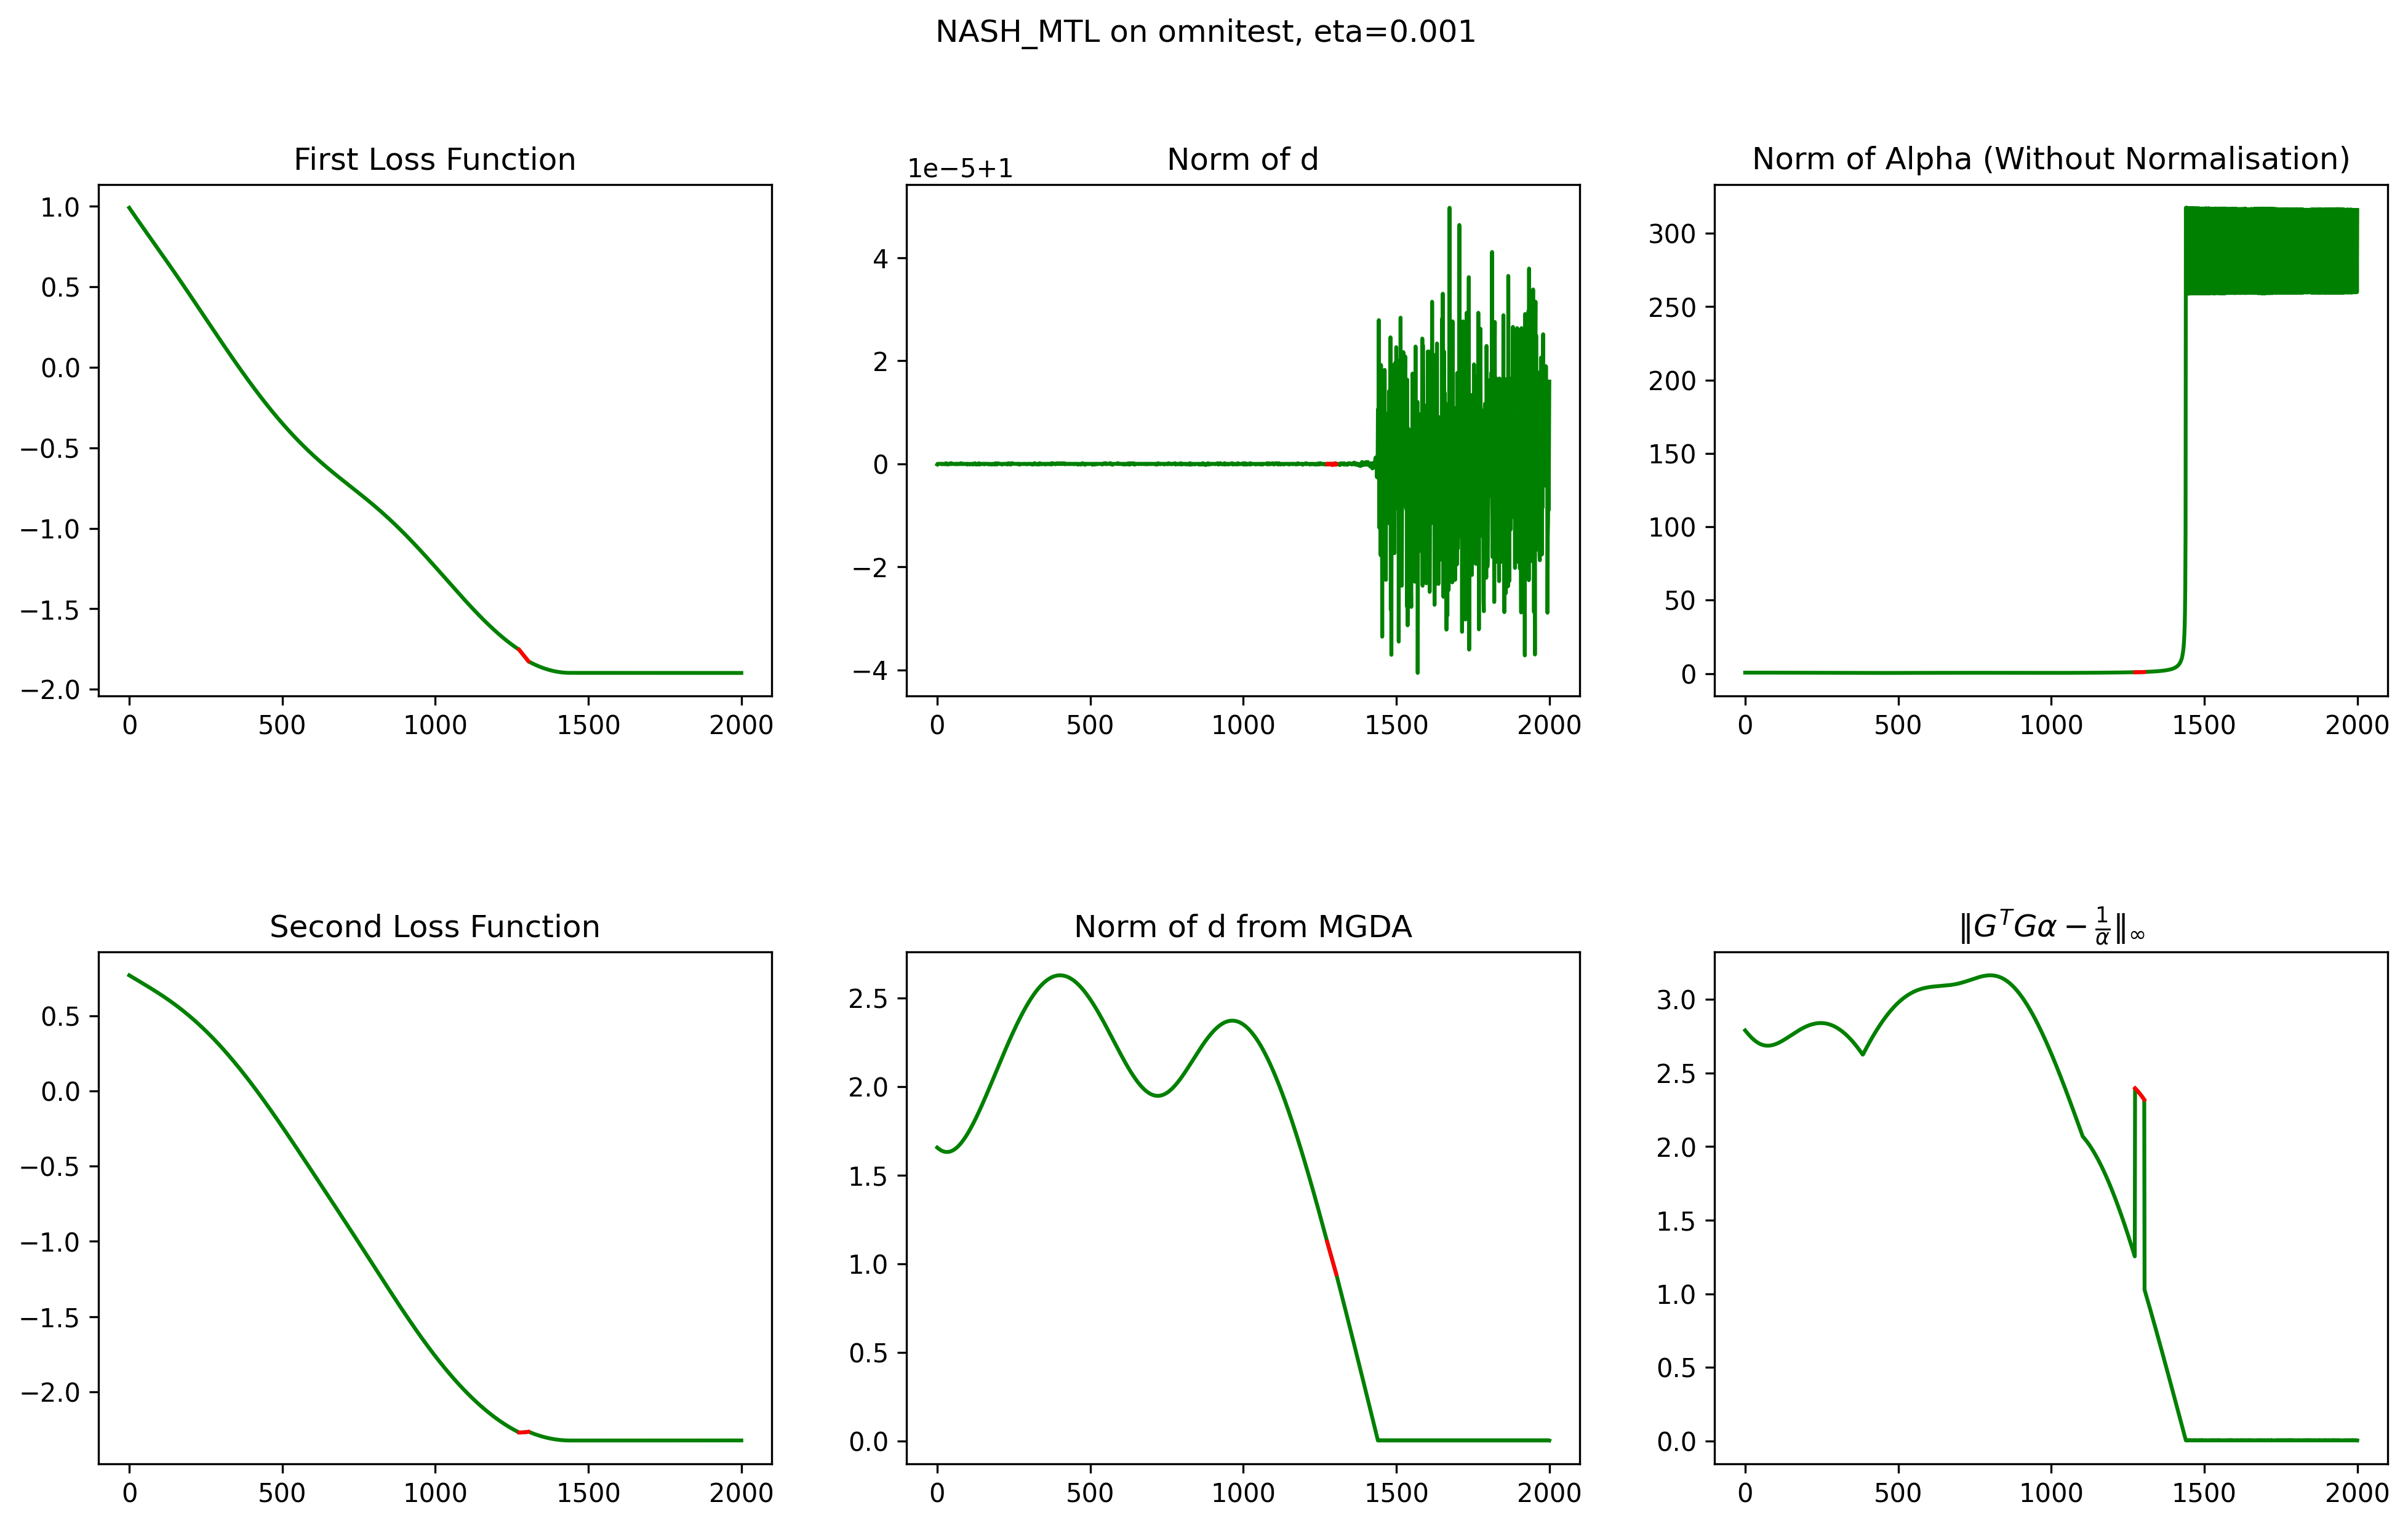
\includegraphics[scale = 0.4]{src/example5.png}
        \caption{Nash-MTL(original implementation) on Omnitest, learning rate = 0.001, max iteration = 15000, seeds = 48. Red section indicates where the minimization problem is unbounded.}\label{nash_mtl_exp_3}
    \end{figure}   
    From figure \ref{nash_mtl_exp_4}, it can be seen the issue of oscillation is immediately improved. The rational of choosing a cyclical learning rate rather than a decay one is to avoid $x_t$ from converging despite not being Pareto stationary.
            \begin{figure}
        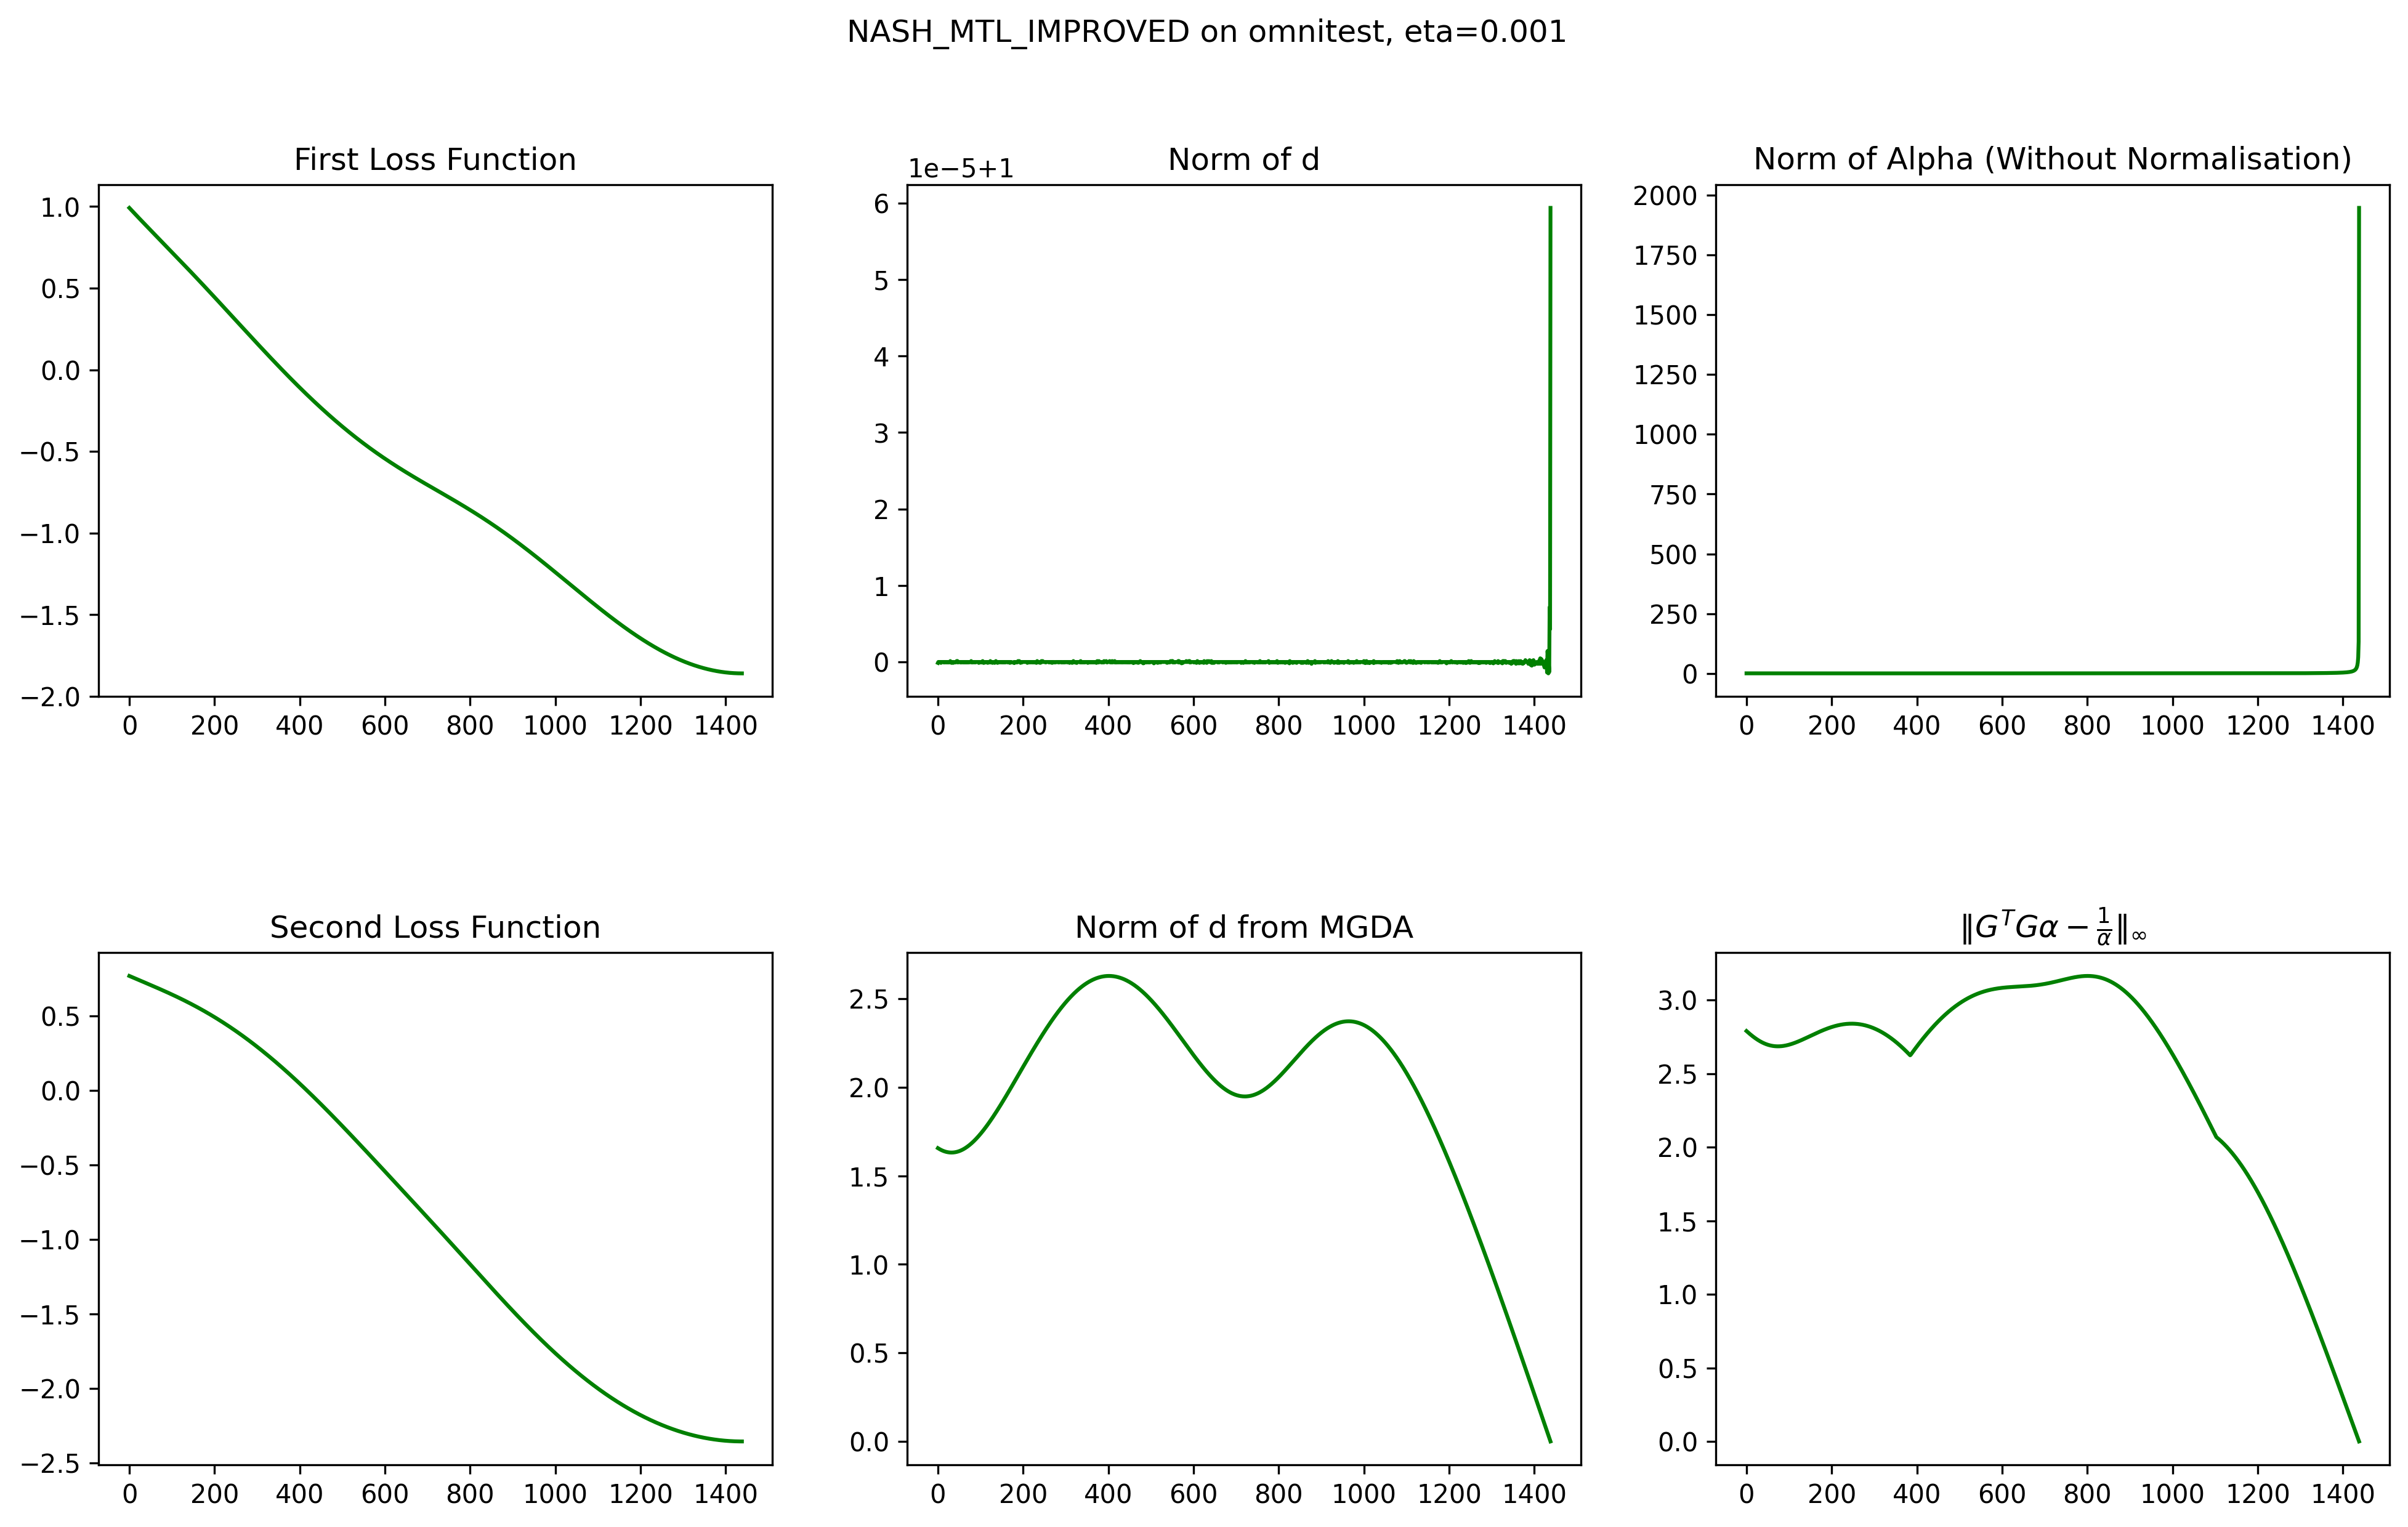
\includegraphics[scale = 0.4]{src/example6.png}
        \caption{Improved Nash-MTL on Omnitest, learning rate = 0.001, max iteration = 15000, seeds = 48. Red section indicates where the minimization problem is unbounded.}\label{nash_mtl_exp_4}
    \end{figure}   
    



\section{Fairness Classification Problem}

We will evaluate the performance of each aggregator with a two objective fairness classification problem. A fully connected NN is trained on the Adult dataset. The dataset present the demographic of US citizens and consists of 15 columns, namely age, work class, fnlwgt\footnote{fnlwgt represents the approximate number of citizens in the US having the same demographic.}, education, education number\footnote{The level of education is numerically represented in a scale from 0 to 16.}, martial status, occupation, relationship, race, sex, country, work time, capital gain, capital loss, and income level\footnote{divided into two classes : "less tof equal to 50K" and "more than 50K"}. A fully connected NN will be trained to predict the income level of a person with two loss functions: the cross-entorpy loss and the DEO loss (more detailed given in appendix). 


    \section{Appendix : Derivation of Nash-MTL Minimization problem}
    In the process of carrying out Nash-MTL, one needs to find the solution of
    \begin{equation*}
    G^T G \alpha = \frac{1}{\alpha},
    \end{equation*}
    where $\frac{1}{\alpha}$ represents the vector $\begin{pmatrix} \frac{1}{\alpha_1} & \frac{1}{\alpha_2} & \cdots & \frac{1}{\alpha_n} \end{pmatrix}^T$.

    To allow the computer to solve the equation, we need to turn it into a minimization problem. Taking the logarithm,
    \begin{align*}
    G^T G \alpha &= \frac{1}{\alpha} \\
    \log(\alpha_i) + \log(\beta_i(\alpha)) &= 0
    \end{align*}
    for any $i \in \{1, 2, \dots, n\}$, where $G = \begin{pmatrix} g_1 & g_2 & \cdots & g_n \end{pmatrix}$ and $\beta_i(\alpha) = g_i^T G \alpha$.

    Define $\varphi_i(\alpha) = \log(\alpha_i) + \log(\beta_i(\alpha))$ and $\varphi(\alpha) = \sum_i \varphi_i(\alpha)$. Parsing into a minimization problem, we have
    \begin{align*}
    \text{Minimize } & \varphi(\alpha) \\
    \text{with constraints } & -\varphi_i(\alpha) \leq 0, \alpha_i \geq 0
    \end{align*}
    for any $i \in \{1, 2, \dots, n\}$.

    Empirical results show that
    \begin{align*}
    \text{Minimize } & \varphi(\alpha) + \sum_i \beta_i(\alpha) \\
    \text{with constraints } & -\varphi_i(\alpha) \leq 0, \alpha_i \geq 0
    \end{align*}
    yields better results. However, the objective function is no longer convex. Hence, we approximate $\varphi_i$ with the second-order Taylor polynomial
    \begin{equation*}
    \tilde{\varphi}(\alpha_t) = \varphi(\alpha_{t-1}) + \nabla \varphi(\alpha_{t-1})(\alpha_t - \alpha_{t-1}).
    \end{equation*}
    Computing $\nabla \varphi(\alpha_{t-1})(\alpha_t - \alpha_{t-1})$, we have
    \begin{align*}
    \frac{\partial \varphi}{\partial \alpha_j} &= \frac{\partial}{\partial \alpha_j} \sum_i \log(\alpha_i) + \log(g_i^T G \alpha) \\
    &= \frac{1}{\alpha_j} + \sum_i \frac{g_i^T g_j}{g_i^T G \alpha} \\
    &= \frac{1}{\alpha_j} + \sum_i \frac{(G^T G)_{ji}}{\beta_i(\alpha)} \\
    &= \left( \frac{1}{\alpha} + G^T G \frac{1}{\beta(\alpha)} \right)_j \\
    \nabla \varphi(\alpha_{t-1})^T (\alpha_t - \alpha_{t-1}) &= \left\langle \frac{1}{\alpha_{t-1}} + G^T G \frac{1}{\beta(\alpha_{t-1})}, \alpha_t - \alpha_{t-1} \right\rangle
    \end{align*}
    Since $\varphi(\alpha_{t-1})$ is a constant, we can drop the term in the minimization problem
    \begin{align*}
    \text{Minimize } & \nabla \varphi(\alpha_{t-1})^T (\alpha_t - \alpha_{t-1}) + \sum_i \beta_i(\alpha) \\
    \text{with constraints } & -\varphi_i(\alpha_t) \leq 0, \alpha_t^i \geq 0,
    \end{align*}
    where we iterate the process several times.
  
   


    \section{Appendix : DEO loss}

    Let $\mc X$ be the feature space, and $f:\mc X\to [0,1]$ classifies the income level. We define the Difference of Equality of Opportunity (DEO) index as 
    \begin{equation*}
        DEO(x) = \frac{1}{N}\sum_{a = 1, y= 1}\mathbb 1_{f(x) > 0} - \frac{1}{N}\sum_{a =  -1, y= 1}\mathbb 1_{f(x) > 0},
    \end{equation*}

    where $a\in \set{-1,1}$ represents the sex of a particular person. The underlying assumption is that the sex of a person should have minimal influence on a person's income level. Ideally, if $f$ is completely fair, the DEO index should be approximately zero. To turn the DEO into a loss function we can train on, we write it as 
    \begin{equation*}
        \widehat{DEO}(x) = \frac{1}{N}\| \sum_{a = 1, y= 1}\tanh(c (f(x)_+) - \sum_{a =  -1, y= 1}\mathbb \tanh(c (f(x)_+)\|,
    \end{equation*}
    where $c$ is a constant equal to one by default.
\end{document}